\documentclass[11pt]{article}
\usepackage[dvipsnames]{xcolor}
\usepackage[T1]{fontenc}
\usepackage{mathtools}
\usepackage[french]{babel}
\usepackage{amsmath,amssymb,amsthm}
\usepackage{framed}
\usepackage{lmodern}
\usepackage{utils}
\usepackage{pdfpages}
\usepackage{irif}

\newcommand*{\ZZ}{n\Z \x n\Z}


\begin{document}
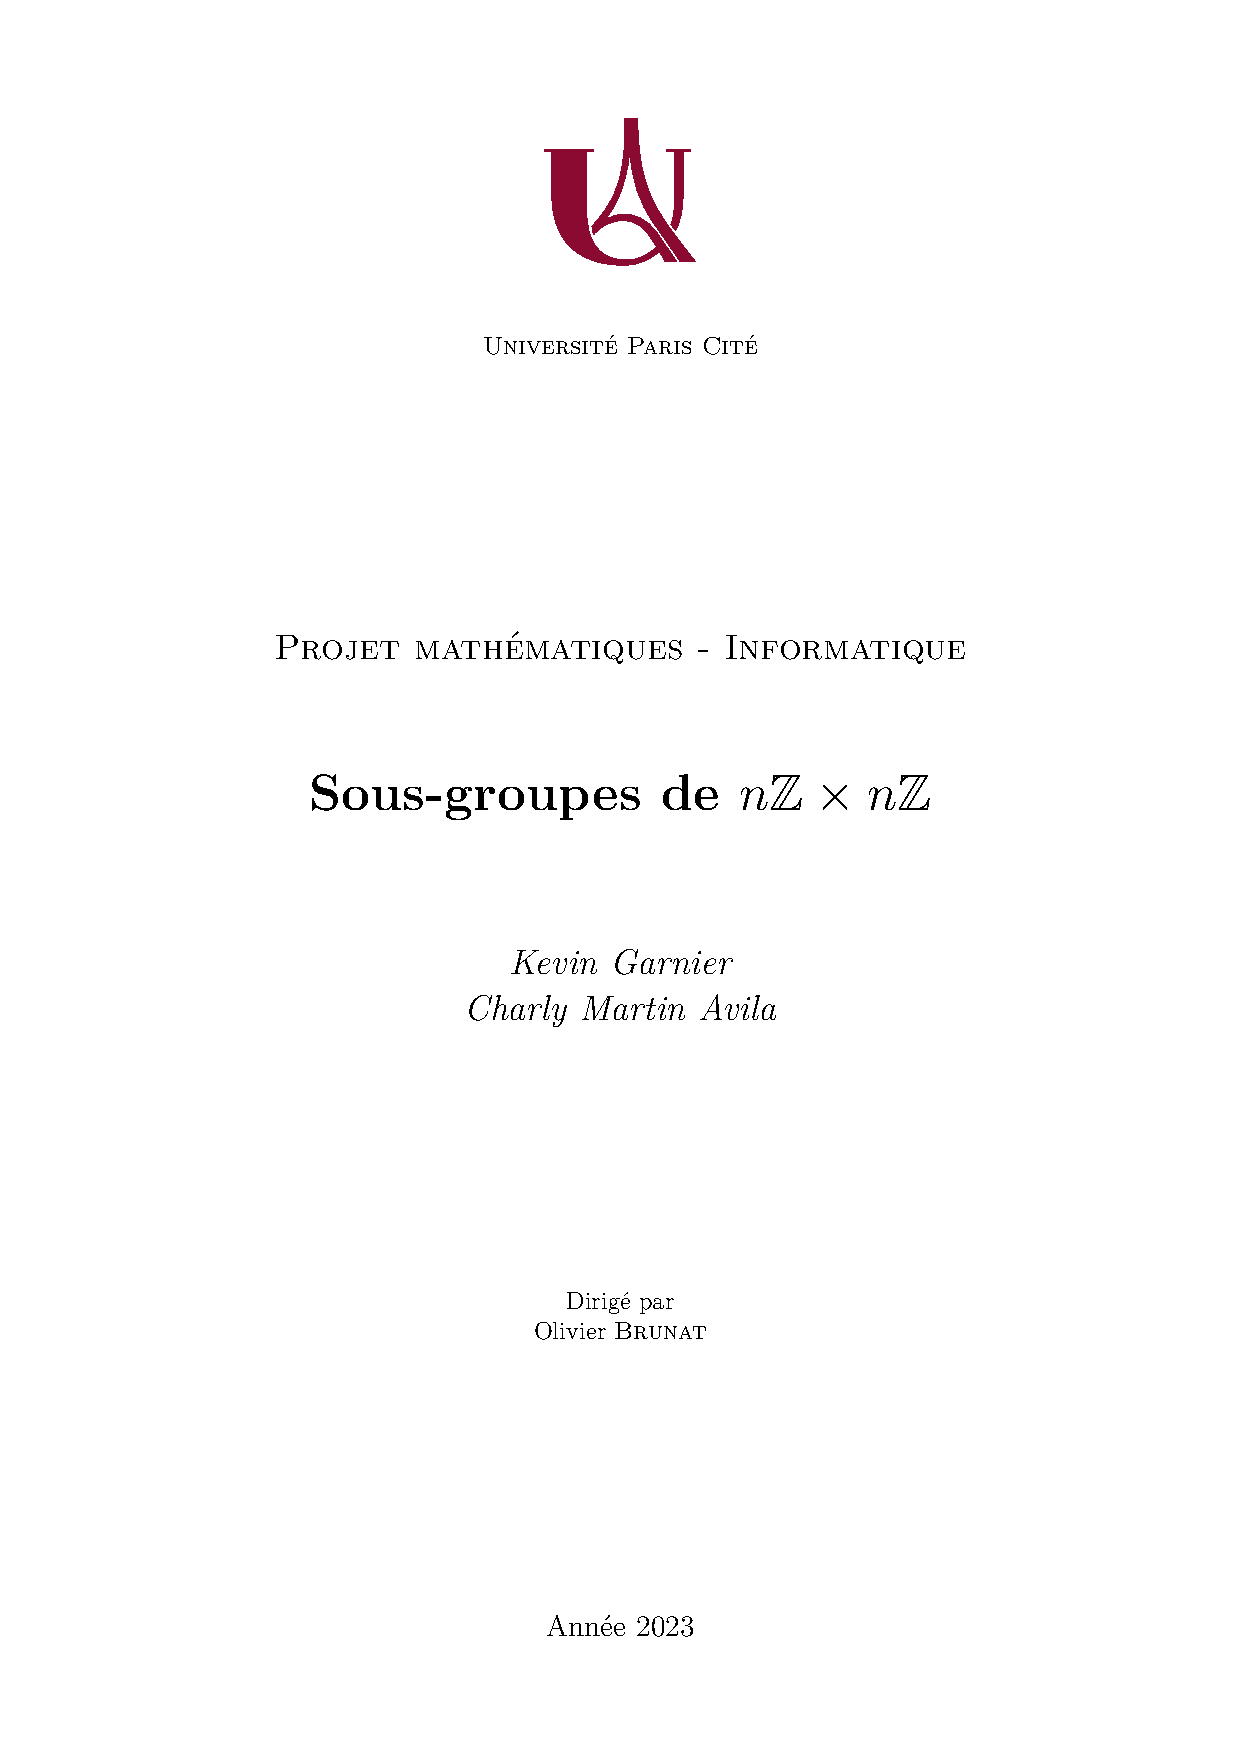
\includepdf{title.pdf}
\tableofcontents

\newpage

\section{Introduction}
	Il est très facile de décrire tous les sous-groupes d'un groupe cyclique
	d'ordre $n$ : il y en a exactement un par diviseur positif de $n$.
	Pourtant, étonnamment, décrire tous les sous-groupes d'un groupe abélien
	est en général un problème difficile.\\
	Dans ce projet, nous nous se proposons de considérer cette question pour le groupe $\ZZ$.

	D'un point de vue théorique, nous mettrons en avant la générations et la caractérisations de \\
	sous-groupes grâce aux vecteurs colonne des matrices à coefficients entier et en particulier aux formes
	normales de Hermite. Nous montrerons aussi une formule permettant de les compter.

	D'un point de vue pratique, nous créerons un programme \textsc{OCaml} capable de générer les\\
	sous-groupes de $\ZZ$ ainsi que leur treillis à partir d'un entier donné en paramètres.


\section{Simplification du problème ?}
% lemme des restes chinois, algorithme nombre premier, decomposition nombre premier

\section{Matrices à coefficients entier et forme normales de Hermite}

% TODO : ajouter demo en rapport avec les matrice im AQ= im A etc
%

\section {Generation et Enumeration des sous-groupes}
%preuve sur la bonne forme de forme normale de Hermite
%preuve sur le calcul du nombre de sous-groupe

\section {Quelques résultats}

\end{document}
